\chapter{Materials and Methods} \label{chap:2}

    All mentioned tools were installed by the Conda package distribution system version 2-2.4.0 (Miniconda) for a easier replication of the results \autocite{Conda}. By the use of Conda, Python packages and full software tools can be installed into environments without touching the system by single commands, making installation of many tools easy and fast. Therefore by execution of the Unix-Shell commands in \autoref{sec:2.1} the same environment can be created as it was used for this project.
    %nochmal conda 
    
    For complete replication of the results the file structure for the \textit{script.sh} needs to be recreated in Unix-Shell by:
    
    \begin{lstlisting}[language=sh]
mkdir -p {Scripts,A/{01_PB2,02_PB1,03_PA,04_HA,05_NP,06_NA,07_MP,08_NS},B/{01_PB1,02_PB2,03_PA,04_HA,05_NP,06_NA_NB,07_M1_BM2,08_NS},C/{01_PB2,02_PB1,03_P3,04_HE,05_NP,06_M1_CM2,07_NS}}\end{lstlisting}  

    The \textit{script.sh} needs to be placed into %\DD{eher "placed into", "moved" ist etwas banal} 
    the root of the structure on the same level as the folders \textit{Scripts}, \textit{A}, \textit{B} and \textit{C}. All other files needs to be moved to the \textit{Scripts} folder. 

    After recreation the up to date sequences for every segment of every desired type must be retrieved from the \gls{IRD} by entering
    
    \begin{enumerate}[noitemsep]
        \item \textit{SEARCH DATA}
        \item \textit{Search Sequences}
        \item \textit{Nucleotide Sequences}
        \begin{enumerate}[noitemsep]
            \item \textit{Data Type: Genome Segments}
            \item \textit{Virus Type:} $X$
            \item \textit{Complete Genome: Complete Genome Only}
            \item \textit{Select Segments:} $Y$
            \item \textit{Complete:} $Y$
        \end{enumerate}
        \item \textit{search}
        \item \textit{download}
    \end{enumerate}
    
    download the files and move them to the respective folder in the file structure.

    The tools in the pipeline of the \autoref{sec:2.2} were executed on every segment of the selected Influenza type. Data was obtained from the \gls{IRD} on 13.06.2019 \autocite{IRD}. The final goal %\DD{"target" ist hier gefuehlt nicht so passend, eher "goal" oder sowas} 
    of the \autoref{sec:2.2} pipeline is to rate the used clustering algorithms based on vector calculations, as well as a visualization of the evolutionary relationship and clustering differences of the genomes to every segment of the selected Influenza type. Possible secondary structures are furthermore predicted by VeGETA in the pipeline and to be validated.% \DD{der ganze Satz ist etwas komisch, wuerde nicht mit "furthermore" anfangen}. 
    %\vspace{\baselineskip}
    %The pipeline of the \nameref{sec:2.3} aims to build a optimized database of the selected influenza type(s) containing informations like the names of the segments related to one specific influenza strain, as well as the country, subcountry, city and year of the outburst and the 5'-\gls{UTR}, \gls{ORF} and 3'-\gls{UTR} sequences of the related segments. After building of the database the comprehensive secondary structure of one specific query is calculated and visualized. The query returns a FASTA file for each Influenza type containing all pseudo genomes from existing strain variations build from the related \gls{UTR} regions.
    %Grafik vom rating
    
\section{Conda preparations} \label{sec:2.1}
    
    In the following, the used conda environments and related tools are listed as Unix-Shell commands. The names of the listed conda environments match the used environments in the pipelines and are necessary for execution without changing the pipeline scripts. 
    
    %\begin{lstlisting}[language=sh, caption=Conda Preparations]
    \begin{lstlisting}[language=sh]
conda config --add channels defaults
conda config --add channels bioconda
conda config --add channels conda-forge
conda config --add channels r

conda create -n projektarbeit
conda activate projektarbeit

conda install ruby
conda install cd-hit
conda install mafft
conda install raxml
conda install newick_utils
conda install viennarna
conda install parallel
conda install jalview

conda deactivate

git clone https://github.com/klamkiew/vegeta.git
export PATH="$HOME/vegeta/bin:$PATH" 
    #include in .Bashrc or .profile for permanent PATH modification 

conda create -n vegeta python=3.6
conda activate vegeta

conda install -c pip
conda install -c cd-hit
conda install -c mafft
conda install -c locarna
conda install -c glpk

pip install numpy biopython colorlog umap-learn hdbscan docopt scipy

conda deactivate \end{lstlisting}  

\section{Project pipeline} \label{sec:2.2}
    
    A visual summary of the full pipeline is shown in \autoref{fig:2.1}. The pipeline can be executed by the following Bash script. For execution of all Bash scripts GNU Bash is used in version 5.0.17(1)-release \autocite{Bash}.
    
    \begin{leftbar}
        \textbf{script.sh}
        \begin{nstabbing}
            \qquad \= \kill
        
            -p \> [number of processes]\\
            
            -i \> [path input directory]
        \end{nstabbing}
    \end{leftbar}

    %\begin{lstlisting}[language=sh, caption=Pipeline Execution]
    \begin{lstlisting}[language=sh]
cd Projektarbeit/Cluster/
bash -i script.sh -p 8 -i B/ > .log\end{lstlisting}
    
    The pipeline was only executed on \gls{IBV}. By expanding the command with \colorbox{backcolour}{-i A/ -i C/}, the pipeline can be used on every segment from all Influenza types including \gls{IAV} and \gls{ICV}. The \colorbox{backcolour}{-p} option changes the number of parallel processes for used tools and can be changed for performance reasons.
    
\subsection{Preparation of sequences} \label{subsec:2.2.1}

    The FASTA file containing the segment sequences needed to be prepared by deleting duplicates, checking of sequences direction (positive or negative strand), extracting 500 random sequences (to keep a rational calculation time) and building a sequence alignment from the 500 sequences.

    \begin{leftbar}
        \textbf{cd-hit-est}
        \begin{nstabbing}
            \qquad \= \kill
        
            -M \> [memory limit]\\
        
            -s \> [length difference cutoff]\\
            
            -C \> [sequence identity threshold]\\
            
            -T \> [number of processes]\\
        
            -i \> [path input FASTA]\\
            
            -o \> [path output FASTA]
        \end{nstabbing}
    \end{leftbar}
    
    \begin{figure}[!hbt]
        \centering
        \fbox{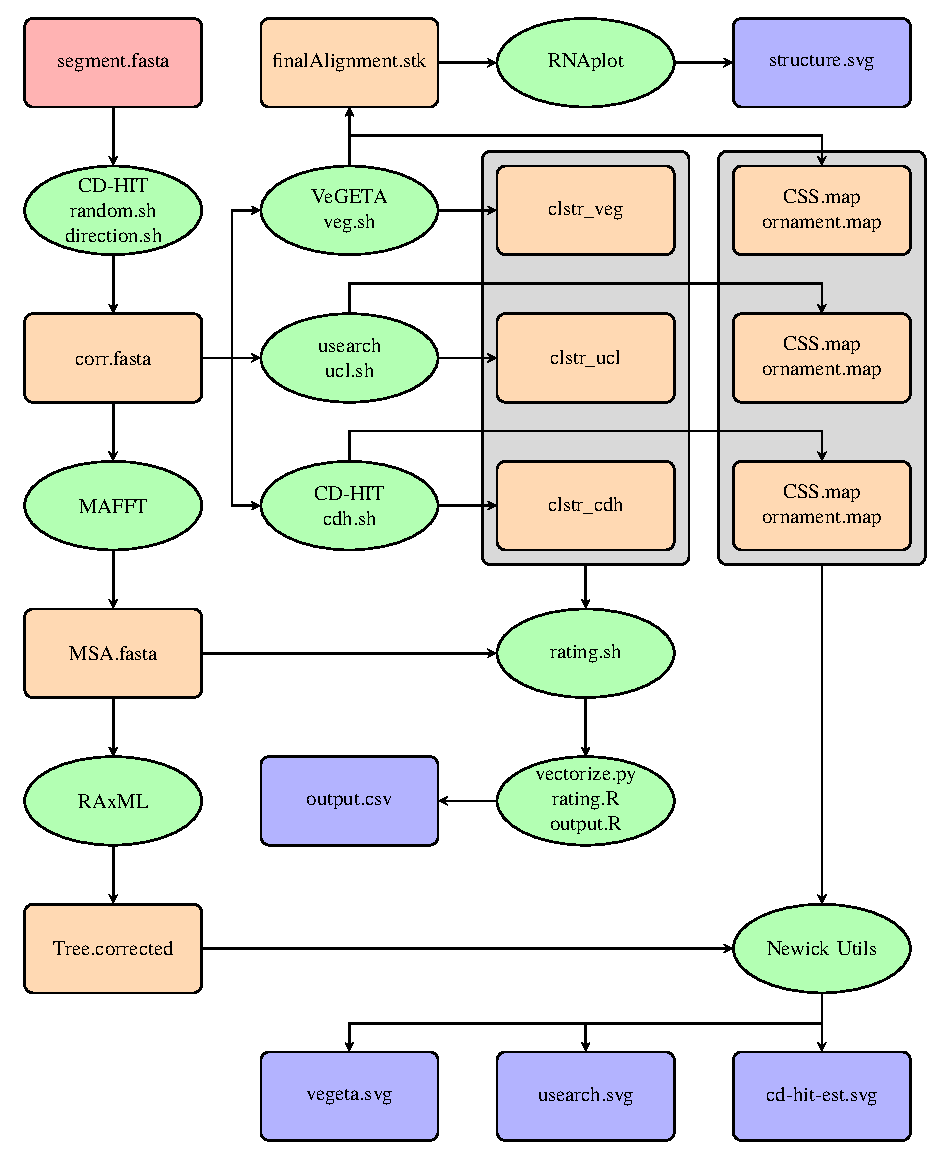
\includegraphics[width=\dimexpr\textwidth-2\fboxsep-2\fboxrule, page=1]{Figures/Projektarbeit_Tikz.pdf}}
        \caption[Project pipeline]{\textbf{Project pipeline.} Visual representation of the described pipeline. Filenames boxed with red coloring are the input for the pipeline. Results are boxed in blue. The used tools described in the following are circled in green. If more than one tool is inside one circle the tools interact with each other or were used simultaneously. Interim results resulting from the used tools are colored in orange. Interim results inside a grey box pointing to a tool are used as input together.}
        \label{fig:2.1}
    \end{figure}
    
    %\DD{bei mir war die eine Haelfte auf Seite 7, dann das Bild, dann alles ab "-i". schaut etwas komisch aus, schau mal ob du das irgendwie ohne Unterbrechung hinbekommst. evtl ne figure draus machen? Oder zumindest das workflow bild dahinter? Wenn es auf ner neuen Seite weitergeht ist es noch ok, aber ne Grafik dazwischen ist irgendwie dof.}
    Deletion of duplicate sequences were realised by CD-HIT version 4.8.1 using parameters to ensure that only duplicates were deleted that have a sequence identity of 100\% and the same length by using \colorbox{backcolour}{-C 1.0} and \colorbox{backcolour}{-s 1.0}. Thus no shorter sequences or sequences with single nucleotide polymorphisms or other differences were deleted. Resulting from this execution, a FASTA file named \textit{unique.fasta} was created \autocite{CD-HIT}.  
    
    \begin{leftbar}
        \textbf{random.sh}
        \begin{nstabbing}
            \qquad \= \kill
        
            -i \> [path input FASTA]\\
        
            -o \> [path output FASTA]\\
            
            -n \> [max. number of random sequences]
        \end{nstabbing}
    \end{leftbar}
    
    For randomization a Bash script was used to first mark every sequence in the \textit{unique.fasta} with a sequential number and then generate 500 random but unique numbers between one and the number of sequences in the file. Based on the 500 random numbers the complete sequences with header matching these numbers were copied to a new FASTA file named \textit{rndm.fasta}. Every sequence from the original file was copied if the original FASTA contained less than 500 sequences. 
    
    \begin{leftbar}
        \textbf{direction.sh}
        \begin{nstabbing}
            \qquad \= \kill
        
            -i \> [path input FASTA]\\
        
            -o \> [path output FASTA]
        \end{nstabbing}
    \end{leftbar}
    
    The correction of the sequence direction was, like the randomization, implemented by a Bash script. Every sequence from the FASTA file containing the random sequences were examined. The sequences in original and reverse transcribed direction as well as with one and two missing nucleotides at the sequence start in original and reverse transcribed direction were split in chunks of three nucleotides. These chunks in the six possible variations were translated to \glspl{AA}. Every possible reading frame can be evaluated to find the longest \gls{ORF}. The sequence variation containing the longest \gls{ORF} in Influenza genomes has the highest possibility to match the real sequence direction. In case the direction wasn't the original sequence direction, the original sequence without missing nucleotides was reverse transcribed and copied to a new FASTA file named \textit{corr.fasta} otherwise the original sequence without missing nucleotides was copied.
    
    \begin{leftbar}
        \textbf{mafft}
        \begin{nstabbing}
            \qquad\qquad\qquad \= \kill
        
            -{}-{}auto \> automatic options (switch)\\
        
            -{}-{}reorder \> aligned output order (switch)\\
            
            -{}-{}quiet \> don't show progress (switch)\\
            
            -{}-{}thread \> [number of processes]\\
            
            \> [path input FASTA]\\
            
            > \> [path output alignment]
        \end{nstabbing}
    \end{leftbar}
    
    MAFFT version v7.471 was then used on the \textit{corr.fasta} file to build a \gls{msa} named \textit{MSA.fasta} with standard options plus reordering the sequences by option \colorbox{backcolour}{-{}-{}reorder} \autocite{MAFFT}. 
    
    \begin{leftbar}
        \textbf{jalview}
        \begin{nstabbing}
            \qquad\qquad\qquad \= \kill
        
            -{}nodisplay \> don't show GUI (switch)\\
        
            -{}colour \> [colorscheme]\\
            
            -{}open \> [path input alignment]\\
            
            -{}svg \> [path output svg]
        \end{nstabbing}
    \end{leftbar}

    The sequence alignment was afterwards visualized by Jalview version 11.0.8-internal to have the possibility to examine differences in regions with noticeable structures. As a coloring scheme the standard nucleotide scheme was used and saved as \textit{MSA.svg} \autocite{Jalview}.

\subsection{Clustering of sequences} \label{subsec:2.2.2}

    The sequences from the file produced by the preparation steps \textit{corr.fasta} was clustered by usearch v11.0.667\_i86linux32, VeGETA v0.3 (alpha) and CD-HIT version 4.8.1 to rate differences in the clustering result \autocite{Usearch, CD-HIT, vegeta}.

    \begin{leftbar}
        \textbf{cd-hit-est}
        \begin{nstabbing}
            \qquad \= \kill
        
            -T \> [number of processes]\\
            
            -n \> [word length]\\
        
            -C \> [sequence identity threshold]\\
        
            -i \> [path input FASTA]\\
            
            -o \> [path output representatives file]
        \end{nstabbing}
    \end{leftbar}
    
    First clustering was performed by CD-HIT with a sequence identity of 95\% by \colorbox{backcolour}{-C 0.95} using the \textit{corr.fasta} as input resulting in files containing the clusters and representatives \autocite{CD-HIT}.
    
    \begin{leftbar}
        \textbf{cdh.sh}
        \begin{nstabbing}
            \qquad \= \kill
        
            -c \> [path input cluster file]\\
        
            -r \> [path input representatives file]\\
            
            -o \> [path output directory]
        \end{nstabbing}
    \end{leftbar}
    
    For the coloring in the evolutionary tree, the cluster and representative files from CD-HIT were restructured and exported as \textit{ornament.map} and \textit{css.map} files by the given Bash script. Simultaneously, the script restructured the information again into a file holding the clusters with related representative and sequence names for the rating step named \textit{clstr\_cdh}.
    
    \begin{leftbar}
        \textbf{usearch}
        \begin{nstabbing}
            \qquad\qquad\qquad \= \kill
        
            -{}cluster\_fast \> [path input FASTA]\\
        
            -{}id \> [sequence identity threshold]\\
            
            -{}centroids \> [path output representatives file]\\
            
            -{}clusters \> [path output cluster files]
        \end{nstabbing}
    \end{leftbar}
    
    Second clustering was performed by usearch with a sequence identity matching the one used with CD-HIT by setting \colorbox{backcolour}{-id 0.95} and with the same FASTA used before \autocite{Usearch}.
    
    \begin{leftbar}
        \textbf{ucl.sh}
        \begin{nstabbing}
            \qquad \= \kill
        
            -c \> [path input cluster files]\\
        
            -r \> [path input representatives file]\\
            
            -o \> [path output directory]
        \end{nstabbing}
    \end{leftbar}
    
    In the same manner as the script before this Bash script restructured and exported the informations given by the usearch files into \textit{ornament.map} and \textit{css.map} files, as well as a custom file named \textit{clstr\_ucl}.
    
    \begin{leftbar}
        \textbf{vegeta}
        \begin{nstabbing}
            \qquad \= \kill
            
            \> [path input FASTA]\\
            
            -o \> [path output dir]\\
            
            -p \> [number of processes]
        \end{nstabbing}
    \end{leftbar}
    
    Third clustering was performed by VeGETA with standard settings on the same FASTA which was used in the other cluster tools \autocite{vegeta}.
    
    \begin{leftbar}
        \textbf{veg.sh}
        \begin{nstabbing}
            \qquad \= \kill
        
            -c \> [path input cluster file]\\
        
            -r \> [path input representatives file]\\
            
            -o \> [path output directory]
        \end{nstabbing}
    \end{leftbar}

    Again, the informations were exported into \textit{ornament.map}, \textit{css.map} and a custom cluster information file named \textit{clstr\_veg} by the given Bash script fitted for execution on VeGETA cluster and representatives files. In conclusion, three \textit{ornament.map} files, three \textit{css.map} files and three cluster information files were generated by the three Bash scripts. One of each for one used clustering tools.

    \begin{leftbar}
        \textbf{RNAplot}
        \begin{nstabbing}
            \qquad \= \kill
            
            -i \> [path input stockholm file]\\
            
            -a \> input is in stockholm format (switch)\\
            
            -o \> [output format]\\
            
            -t \> [layout-type]
        \end{nstabbing}
    \end{leftbar}
    
    The stockholm file created by VeGETA was visualized using RNAplot from the ViennaRNA package version 2.4.15 with svg output settings and circular layout type \colorbox{backcolour}{-t 2} \autocite{Vienna}. 

    \begin{leftbar}
        \textbf{mafft}
        \begin{nstabbing}
            \qquad\qquad\qquad \= \kill
        
            -{}-{}auto \> automatic options (switch)\\
        
            -{}-{}reorder \> aligned output order (switch)\\
            
            -{}-{}quiet \> don't show progress (switch)\\
            
            -{}-{}thread \> [number of processes]\\
            
            \> [path input FASTA]\\
            
            > \> [path output alignment]
        \end{nstabbing}
    \end{leftbar}
    
    To be able to find conserved sequences later, MAFFT was used again with the same settings to calculate the \gls{msa} of the representatives for every tool. 

\clearpage
\subsection{Evolutionary distance analysis} \label{subsec:2.2.3}

    \begin{leftbar}
        \textbf{raxmlHPC-PTHREADS-SSE3}
        \begin{nstabbing}
            \qquad \= \kill
            
            -T \> [number of processes]\\
            
            -N \> [number of alternative runs]\\
            
            -f \> [used algorith]\\
            
            -x \> [integer number]\\
            
            -p \> [random number seed]\\
            
            -m \> [model of substitution]\\
            
            -s \> [path input alignment]\\
            
            -w \> [path output directory]\\
            
            -n \> [name of the output file]
        \end{nstabbing}
    \end{leftbar}
    
    RAxML was used to build trees giving information of the evolutionary distances of the genomes from the MAFFT alignment \textit{MSA.fasta}. Recommended settings from the RAxML manual (\colorbox{backcolour}{-N 100}, \colorbox{backcolour}{-x 1234}, \colorbox{backcolour}{-p 1234} and \colorbox{backcolour}{-m GTRGAMMA}) were used with a custom name \textit{RAxML\_bipartitionsBranchLabels.Tree} for the output file \autocite{RAxML}. 
    \begin{leftbar}
        \textbf{raxml2drawing.rb}
        \begin{nstabbing}
            \qquad \= \kill
            
            \> [path input RAxML tree file]
        \end{nstabbing}
    \end{leftbar}

    For the visualization of the RAxML tree, a Ruby script written by Martin Hölzer was used to shorten the evolutionary distance values in the file itself, for clearer display \autocite{Ruby}.

    \begin{leftbar}
        \textbf{nw\_topology}
        \begin{nstabbing}
            \qquad \= \kill
            
            \> [path input RAxML tree file]\\
            
            > \> [path output RAxML topology file]
        \end{nstabbing}
    \end{leftbar}
    
    To visualize the RAxML tree as a radial cladogram, nw\_topology and nw\_display from the Newick Utilities 1.6 were used \autocite{Newick}.
    
    \begin{leftbar}
        \textbf{nw\_display}
        \begin{nstabbing}
            \qquad \= \kill
            
            -v \> [number of pixels between leaves]\\
            
            -i \> [CSS for inner node labels]\\
            
            -l \> [CSS for leaf node labels]\\
            
            -I \> [position of the inner node label]\\
            
            -w \> [set width or scale]\\
            
            -s \> output as svg (switch)\\
            
            -r \> output as radial tree (switch)\\
            
            -b \> [CSS for branch length labels]\\
            
            -c \> [path input css file]\\
            
            -o \> [path input ornament file]\\
            
            \> [path input RAxML topology file]\\
            
            > \> [path output svg]
        \end{nstabbing}
    \end{leftbar}

    The topological information was generated by nw\_topology and then visualized and saved as svg by nw\_display. The settings used were of decorative nature to generate a clear and readable svg-file. Furthermore, the generated \textit{css.map} and \textit{ornament.map} files from the Bash scripts were used here to color the generated clusters and representatives by usearch, VeGETA and CD-HIT in the radial tree. In conclusion, three different svg-files with the same radial tree but, different coloring were created, one for every used clustering tool with the corresponding clustering of the sequences represented by the color scheme \autocite{Newick}.

\subsection{Rating of clustering quality} \label{subsec:2.2.4}

    To rate the clustering quality of each used clustering tool, a Bash script was used which takes a combined text file containing the custom made cluster information files and the \textit{MSA.fasta} generated in the earlier steps as input.

    \begin{leftbar}
        \textbf{rating.sh}
        \begin{nstabbing}
            \qquad \= \kill
            
            -m \> [path input alignment]\\
            
            -o \> [path output directory]\\
            
            -i \> [path input cluster information file]
        \end{nstabbing}
    
        \begin{leftbar}
            \textbf{parallel}
            \begin{nstabbing}
                \qquad\qquad\qquad \= \kill
                
                -{}-{}keep-order \> keep order of input (switch)\\
                
                -{}-{}progress \> show progress (switch)\\
                
                -{}-{}jobs \> [number of parallel jobs]\\
                
                [command] \> [arguments]
            \end{nstabbing}
        \end{leftbar}
    
        \begin{leftbar}
            \textbf{vectorize.py}
            \begin{nstabbing}
                \qquad \= \kill
                
                \> [path input codon table]\\
                
                \> [path output directory]\\
                
                \> [step size]\\
                
                \> [window size]\\
                
                \> [path input cluster FASTA file]
            \end{nstabbing}
        \end{leftbar}
        
        \begin{leftbar}
            \textbf{rating.R}
            \begin{nstabbing}
                \qquad \= \kill
                
                \> [path input cluster vector file]
            \end{nstabbing}
        \end{leftbar}
    
        \begin{leftbar}
            \textbf{output.R}
            \begin{nstabbing}
                \qquad \= \kill
                
                \> [path input temporary rating files]\\
                
                \> [path output rating file]
            \end{nstabbing}
        \end{leftbar}
    \end{leftbar}    
    
    Based on the clusters generated by the clustering tools, the script calculates a vector for every sequence in the cluster by calculating the distance to the representative of the cluster. This was done by using GNU Parallel 20200722 for multiple executions of a python 3.8.5 script \autocite{Parallel, Python}. The calculation of the distance is based on the differences of the nucleotides at the same positions by a cost function using the length uniformed sequences from \textit{MSA.fasta} (siehe \autoref{tab:2.1}). This was done for every cluster from every clustering tool. 
    
    %change to include silent mutations
    \begin{table}[!htb]
        \centering
        \begin{tabu} to \textwidth{ |C|C|C|C|C|C|C| }
            \hline
             & \textbf{A} & \textbf{C} & \textbf{G} & \textbf{U} & \textbf{N} & \textbf{-}\\
            \hline
            \textbf{A} & 0 & 3 (1) & 2 (1) & 3 (1) & 0 & 3\\
            \hline
            \textbf{C} & 3 (1) & 0 & 3 (1) & 2 (1) & 0 & 3\\
            \hline
            \textbf{G} & 2 (1) & 3 (1) & 0 & 3 (1) & 0 & 3\\
            \hline
            \textbf{U} & 3 (1) & 2 (1) & 3 (1) & 0 & 0 & 3\\
            \hline
            \textbf{N} & 0 & 0 & 0 & 0 & 0 & 3\\
            \hline
            \textbf{-} & 3 & 3 & 3 & 3 & 3 & 0\\
            \hline
        \end{tabu}
    	\caption[Costs used for cluster rating]{\textbf{Costs used for cluster rating.} For conversion of the differences between the representative (nucleotides on top) and the sequences in the cluster (nucleotides left) the given costs were used. If no difference is found, no costs were recorded. \Glspl{SNP} without changing the \gls{AA}, the triplet is coding for, is called silent mutation and rated by the value inside the braces. If the nucleotide changed is still a purin- or still a pyrimidinbase the \gls{SNP} called transition is rated by the cost of value two. In all other cases of \gls{SNP} as well as deletion or insertion it is rated by value three. %\DD{War das die Stelle, die du nochmal überarbeiten wolltest?}
    	}
        \label{tab:2.1}
    \end{table}
   
    Following the calculation of the vectors the bash script executed two scripts using R version 3.6.3. The first one to calculate the \gls{MED}, as well as the \gls{MMD}, for result comparison with different distance functions, on all $m$ vectors related to one cluster together (\autoref{eq:1} and \autoref{eq:2}). The calculation was done by two consecutive summation containing the euclidean or manhattan distance calculation in the middle. That way the distance between all the $m$ vectors were measured by using the distance functions on vector $n$ and $o$ from $m$ and finally divided by the number of calculations necessary.  
    
    \begin{empheq}{alignat = -1}
        &\text{MED} &&= \sum\limits_{n=1}^{m-1} &&\Bigg( &&\sum\limits_{o=n+1}^{m} &&\Bigg( &&\sqrt{\sum\limits_i^j (n_i - o_i)^2} &&\Bigg) &&\Bigg) &&\cdot &&\binom{m}{2}^{-1}\label{eq:1}\\
        \nonumber \\
        &\text{MMD} &&= \sum\limits_{n=1}^{m-1} &&\Bigg( &&\sum\limits_{o=n+1}^{m} &&\Bigg( &&\hphantom{\sqrt{}}\sum\limits_i^j |n_i - o_i| &&\Bigg) &&\Bigg) &&\cdot &&\binom{m}{2}^{-1}\label{eq:2}
    \end{empheq}
    
    This process was repeated for every cluster of every used tool (\autoref{tab:2.3}). The second R script outlines these results for every cluster tool, by calculating the weight of each \gls{MED} of \gls{MMD} and sum them up for every specific tool. This was done by building the product of the \gls{MED} or \gls{MMD} with the fraction of clustersize and total number of used sequences for clustering (\autoref{tab:2.4} and \autoref{eq:3} to \autoref{eq:5}) \autocite{R}.
    
    \begin{table}[!htb]
        \centering
        \begin{tabu} to \textwidth{X[1.25,l]X[1,r]X[1,r]X[1,r]X[1.25,r]}
            \toprule
    		\textbf{tool} & \ltab\textbf{cluster} & \ltab\textbf{MED} & \ltab\textbf{MMD} & \ltab\textbf{cluster size $\bm{m}$}\\
    		\midrule
    		CD-HIT&0&8.901& 65.963 &102\\
            usearch&0&8.922& 66.324 &102\\
            VeGETA&0&6.595& 38.765 &66\\
            VeGETA&1&4.259& 14.588 &17\\
            VeGETA&2&13.318& 88.444 &10\\
            VeGETA&3&6.994& 43.800 &6\\
            VeGETA&4&145.894& 7095.000 &1\\
            VeGETA&5&145.894& 7095.000 &1\\
            VeGETA&6&145.894& 7095.000 &1\\
    		\bottomrule
    	\end{tabu}
    	\caption[Example result from \textit{rating.R}]{\textbf{Example result from \textit{rating.R}.} By execution of \textit{rating.R} the vectors of every sequence in the cluster containing the costs were used to calculate the \gls{MED} inside the cluster.}
        \label{tab:2.3}
    \end{table}
    
    The \gls{MED} and \gls{MMD} of single sequences clusters, were calculated by creating two vectors, one with the highest penalty three in every entry and one with the lowest zero. The distance of these two vectors is the highest possible for the given length. The resulting very high \gls{MMD} and \gls{MED} values punish tools for building of single sequence clusters. %(\autoref{eq:6} and \autoref{eq:7}).
    
    \begin{table}[!htb]
        \centering
        \begin{tabu} to 0.7\textwidth{X[1.25,l]X[1,r]X[1,r]}
    		\toprule
    		\textbf{tool} & \ltab\textbf{MED} & \ltab\textbf{MMD}\\
    		\midrule
    		CD-HIT & 8.901 & 65.963\\
            usearch & 8.922 & 66.324\\
            VeGETA & 10.985 & 247.438\\
    		\bottomrule
    	\end{tabu}
    	\caption[Example result from \textit{output.R}]{\textbf{Example result from \textit{output.R}.} By execution of \textit{output.R} the results from \textit{rating.R} were weighted by the cluster sizes to the total number of sequences and summed up for every tool.}
        \label{tab:2.4}
    \end{table}
    
    \begin{empheq}{alignat = -1}
        &8.901 &&= 8.901 &&\cdot 102 &&\cdot 102^{-1}\label{eq:3}\\
        &8.922 &&= 8.922 &&\cdot 102 &&\cdot 102^{-1}\label{eq:4}\\
        &10.985 &&= 6.595 &&\cdot 66 &&\cdot 102^{-1}\nonumber \\
            &&&+ 4.259 &&\cdot 17 &&\cdot 102^{-1}\nonumber \\
            &&&+ 13.318 &&\cdot 10 &&\cdot 102^{-1}\nonumber \\
            &&&+ 6.994 &&\cdot 6 &&\cdot 102^{-1}\nonumber \\
            &&&+ 145.894 &&\cdot 1 &&\cdot 102^{-1} \cdot 3 \label{eq:5}
    \end{empheq}
    
    % \begin{empheq}{alignat = -1}
    %     &\text{MED} &&= \sqrt{\sum\limits_i^j (3 - 0)^2}\label{eq:6}\\
    %     &\text{MMD} &&= \hphantom{\sqrt{}}\sum\limits_i^j |3 - 0|\label{eq:7}
    % \end{empheq}

\clearpage
\section{Tool versions} \label{sec:2.4}

    The versions of the mentioned tools used in \autoref{sec:2.2} are listed in \autoref{tab:2.2}.

    \begin{table}[!htb]
        \centering
        \begin{tabu} to \textwidth{XX[3]R[2]}
    		\toprule
    		\textbf{Tool} & \textbf{Usage} & \ltab\textbf{Version}\\
    		\midrule
    	    GNU Bash & \nameref{subsec:2.2.1} & 5.0.17(1)-release\\
    	    & \nameref{subsec:2.2.2} & \\
    	    & \nameref{subsec:2.2.4} & \\
    		CD-HIT-EST & \nameref{subsec:2.2.1} & 4.8.1\\
    		& \nameref{subsec:2.2.2} & \\
    		MAFFT & \nameref{subsec:2.2.1} & v7.471\\
    		& \nameref{subsec:2.2.2} & \\
    		Jalview & \nameref{subsec:2.2.1} & 11.0.8-internal\\
    		usearch & \nameref{subsec:2.2.2} & v11.0.667\_i86linux32\\
    		VeGETA & \nameref{subsec:2.2.2} & v0.3 (alpha)\\
    		RNAplot & \nameref{subsec:2.2.2} & 2.4.15\\
    		RAxML & \nameref{subsec:2.2.3} & 8.2.12\\
    		Ruby & \nameref{subsec:2.2.3} & 2.6.6p146\\
    		Newick Utils & \nameref{subsec:2.2.3} & 1.6\\
    		GNU Parallel & \nameref{subsec:2.2.4} & 20200722\\
    		Python & \nameref{subsec:2.2.4} & 3.8.5\\
    		R & \nameref{subsec:2.2.4} & 3.6.3\\
    		\bottomrule
    	\end{tabu}
    	\caption[Tool versions]{\textbf{Tool Versions.} The versions of all the used tools and programming languages in \autoref{sec:2.2}, in order of usage without repetition.}
        \label{tab:2.2}
    \end{table}